\documentclass[a4paper]{article}
\usepackage[left=2cm, right=2cm]{geometry}
\usepackage{lipsum}
\usepackage{tikzpagenodes}
\usepackage{pgfplots}
\usepackage{tikz}
\usepackage{tikz-3dplot}
\usetikzlibrary{arrows,decorations.pathmorphing,backgrounds,positioning,fit,matrix}
\pgfplotsset{compat=1.8}
\usepackage{graphics} % for pdf, bitmapped graphics files
\usepackage{epsfig} % for postscript graphics files
\usepackage[colorlinks=true,citecolor=green]{hyperref}
\usepackage{cite}
\usepackage{amsmath,amssymb,amsfonts}
\usepackage{algorithmic}
\usepackage{graphicx}
\usepackage{url}
\usepackage{cite}
\usepackage{bm}
\usepackage{pbox}
\usepackage{siunitx,booktabs,etoolbox}
\usepackage{ulem}
\usepackage{titling}
\usepackage{float}
%\usepackage{pgf,tikz,pgfplots}
%\pgfplotsset{compat=1.15}
%\usepackage{mathrsfs}

\usetikzlibrary{arrows}

\def\BibTeX{{\rm B\kern-.05em{\sc i\kern-.025em b}\kern-.08em
		T\kern-.1667em\lower.7ex\hbox{E}\kern-.125emX}}
\title{Ex1: Introductory exercise}
\author{Xiao Hu, emails: \url{xiahaa@space.dtu.dk}}
\begin{document}
	\maketitle
	\thispagestyle{empty}
	%\maketitle
	%\clearpage
	\section{Results}
	Results are shown as follows:
		\begin{figure}[htbp]
	\centering
	\includegraphics[width=0.8\textwidth]{./figures/res1.png}
	\caption{Blob detection result. Blobs are detected where the local maximas are detected.}
\end{figure}

\begin{figure}[htbp]
	\centering
	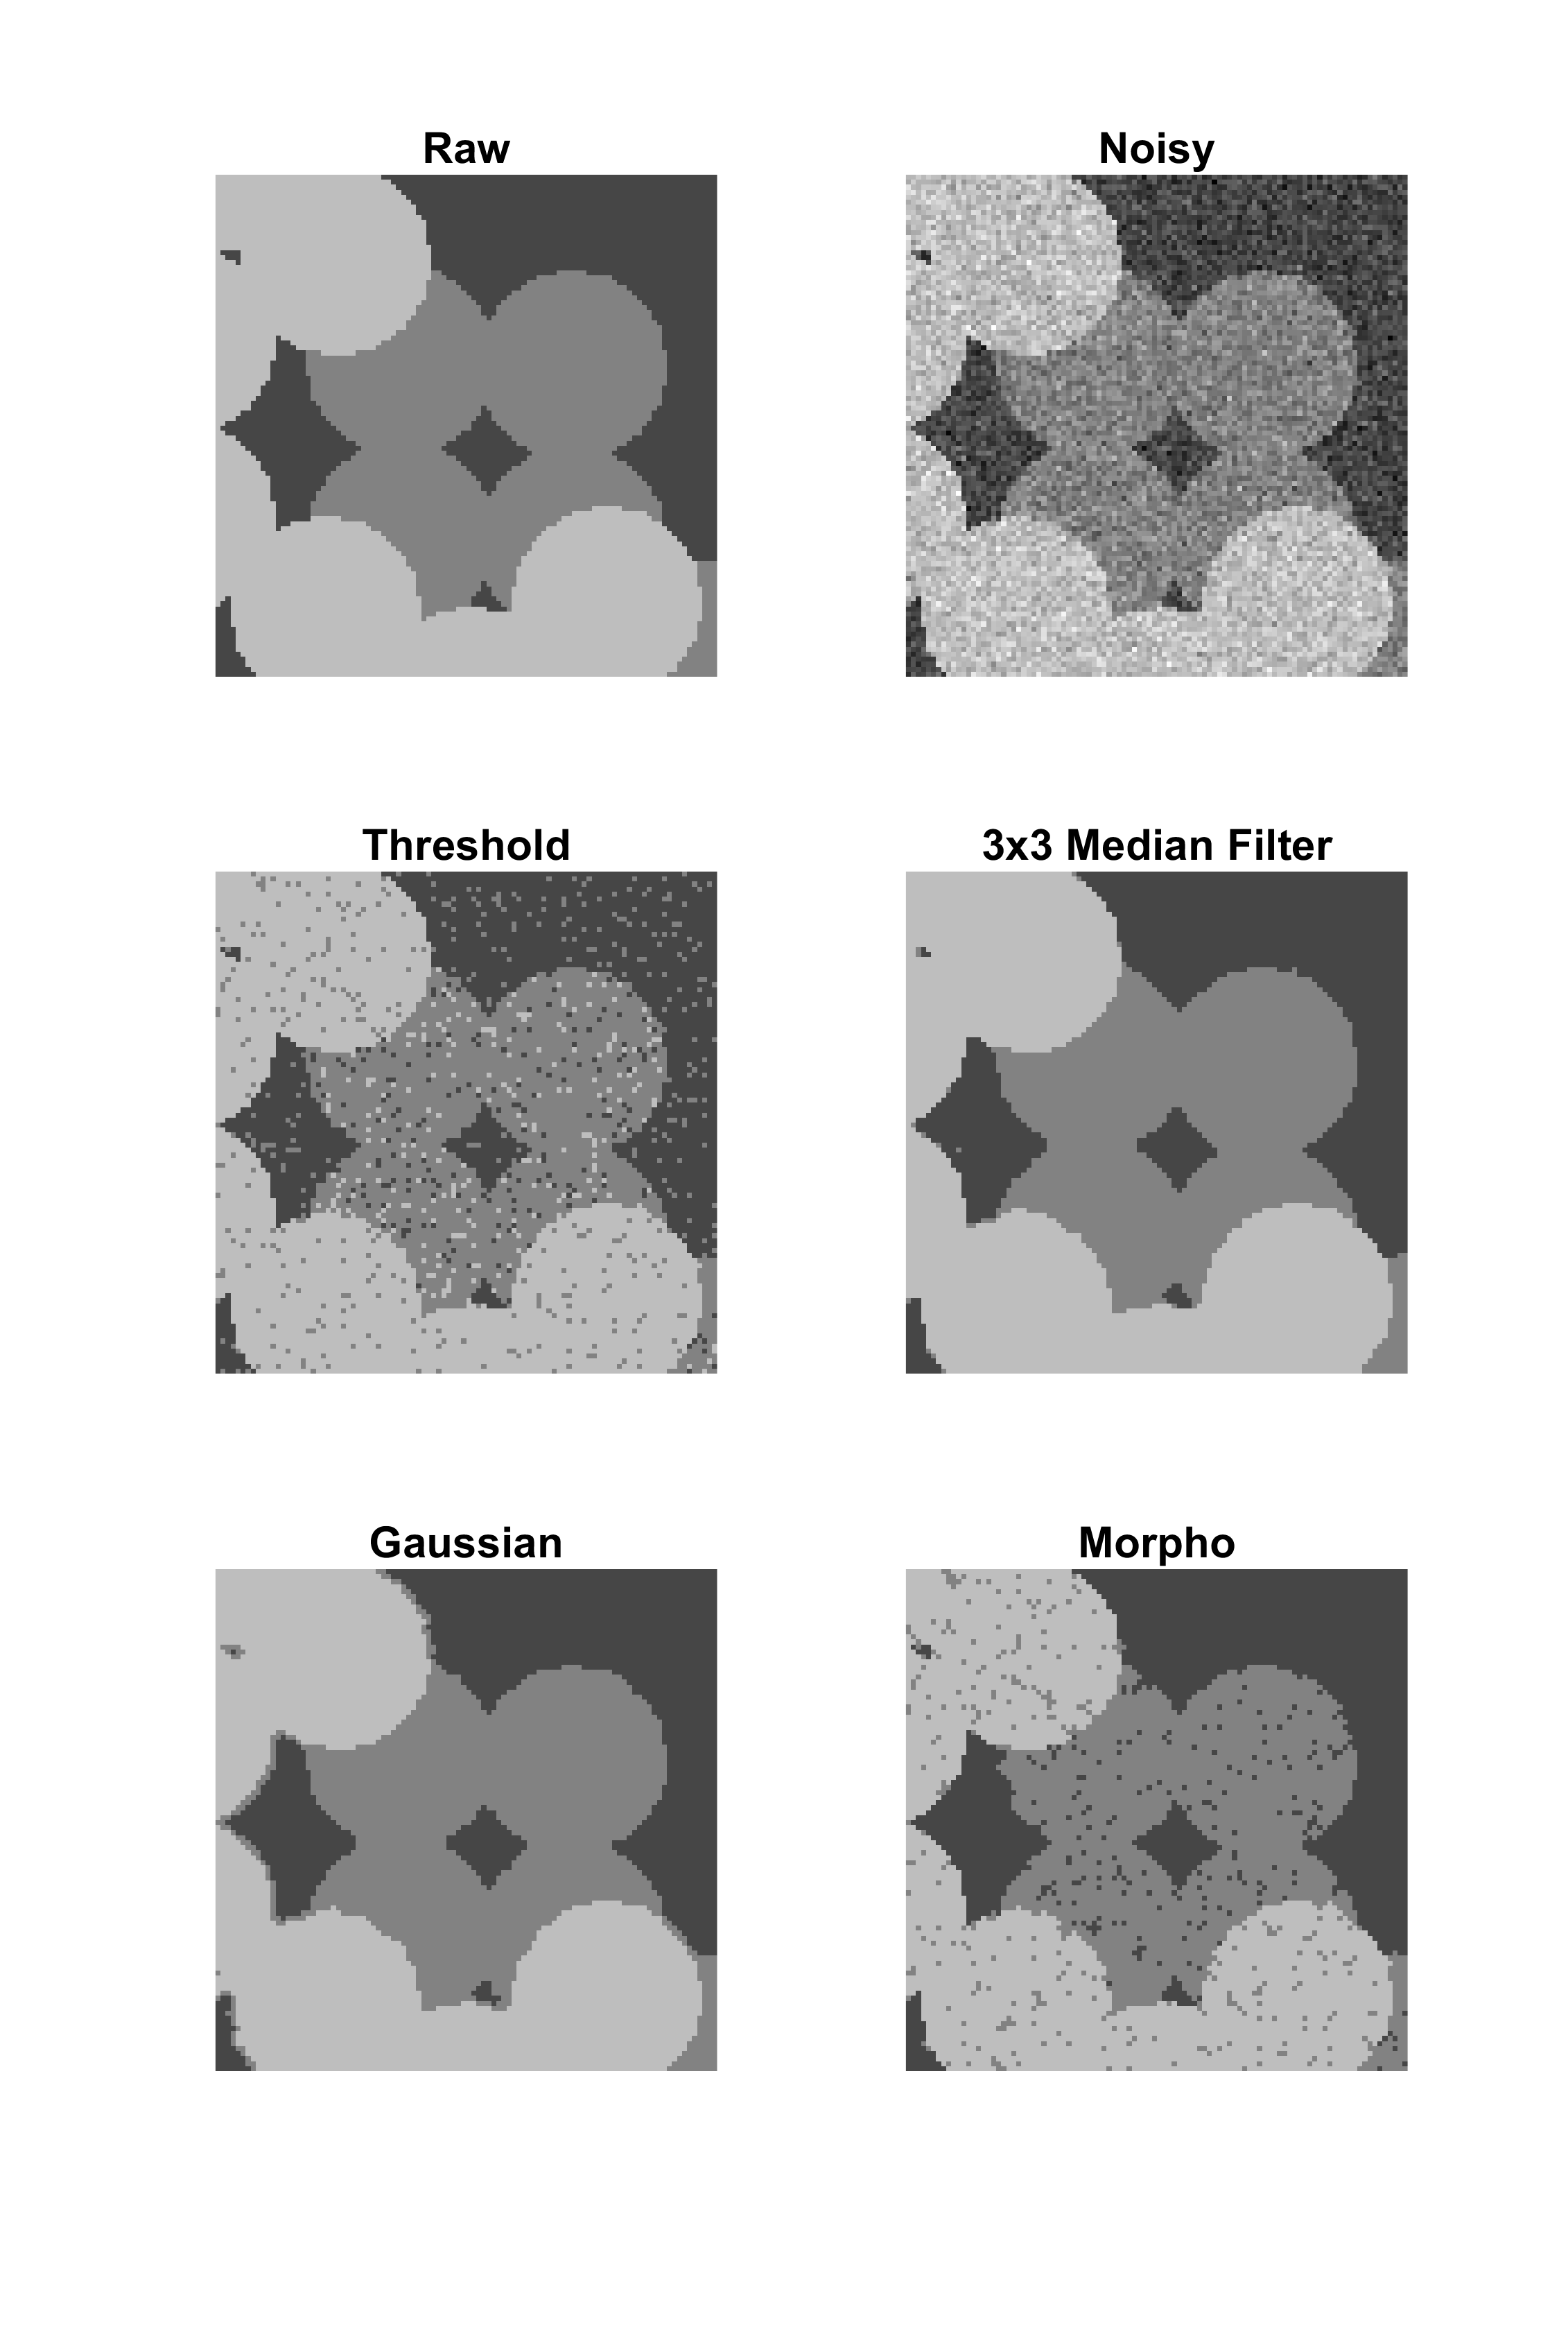
\includegraphics[width=0.8\textwidth]{./figures/res2.png}
	\caption{Blob detection result. Blobs are detected where the local maximas are detected.}
\end{figure}
\begin{figure}[htbp]
	\centering
	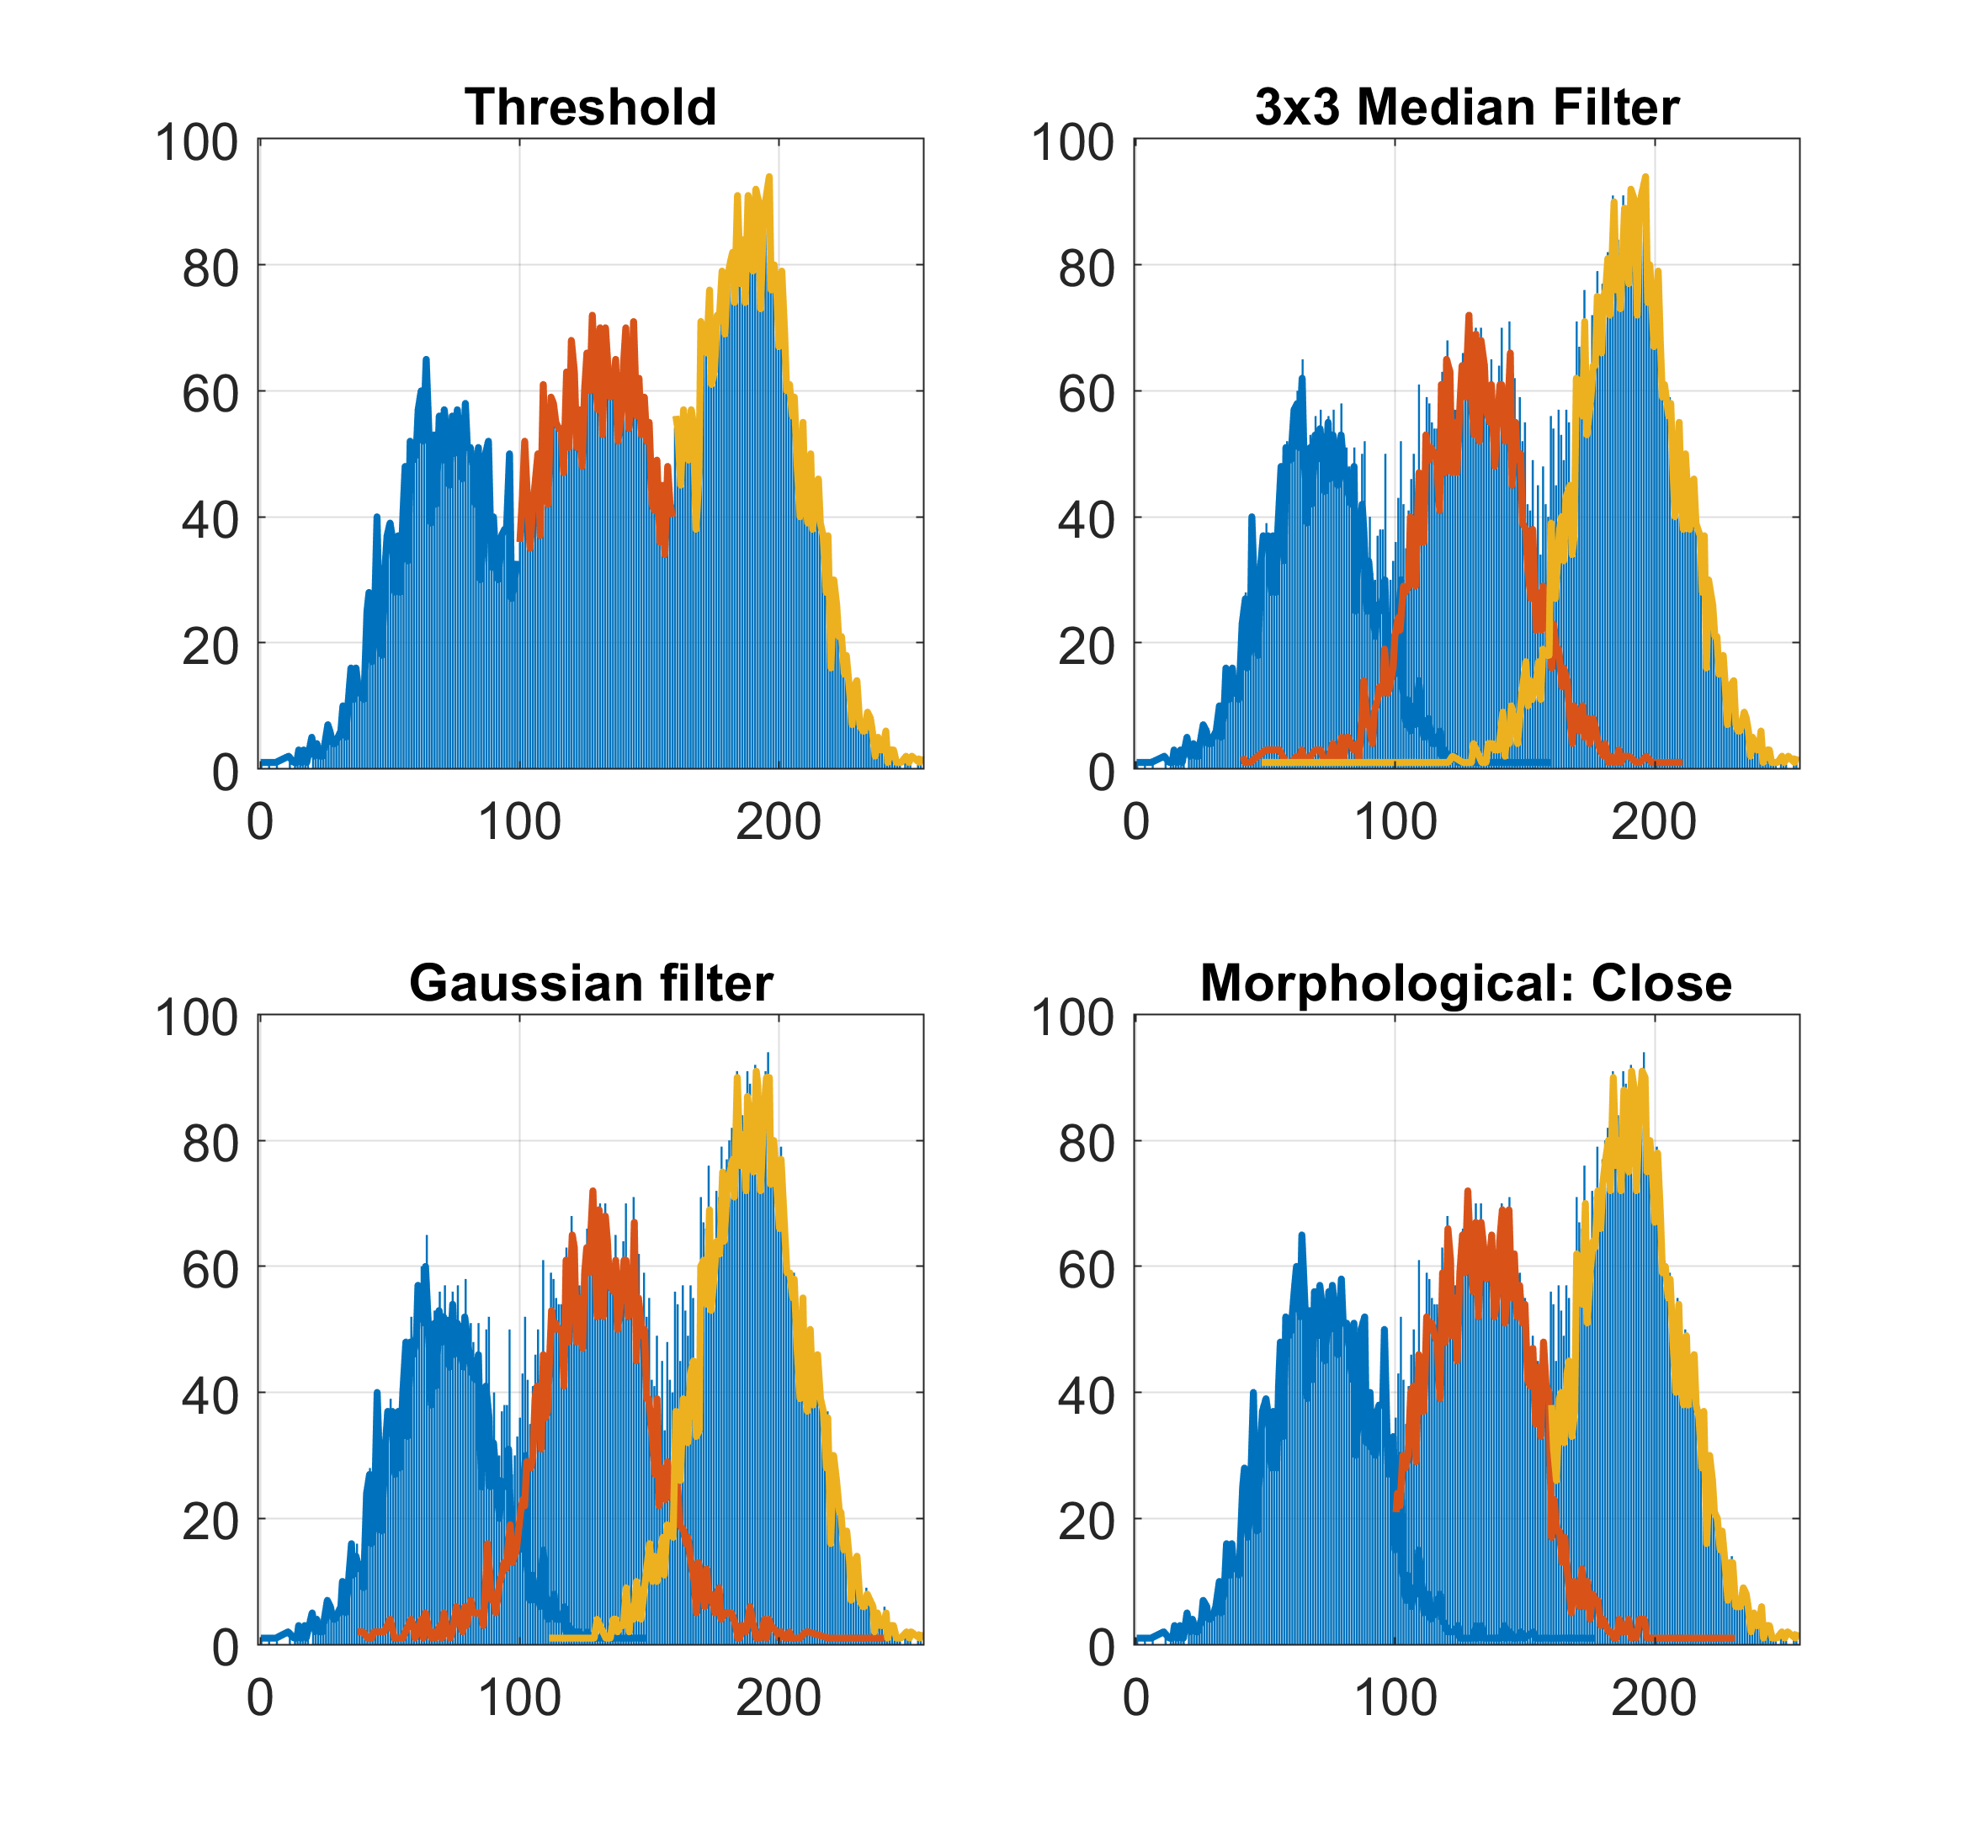
\includegraphics[width=0.8\textwidth]{./figures/res3.png}
	\caption{Blob detection result. Blobs are detected where the local maximas are detected.}
\end{figure}
\begin{figure}[htbp]
	\centering
	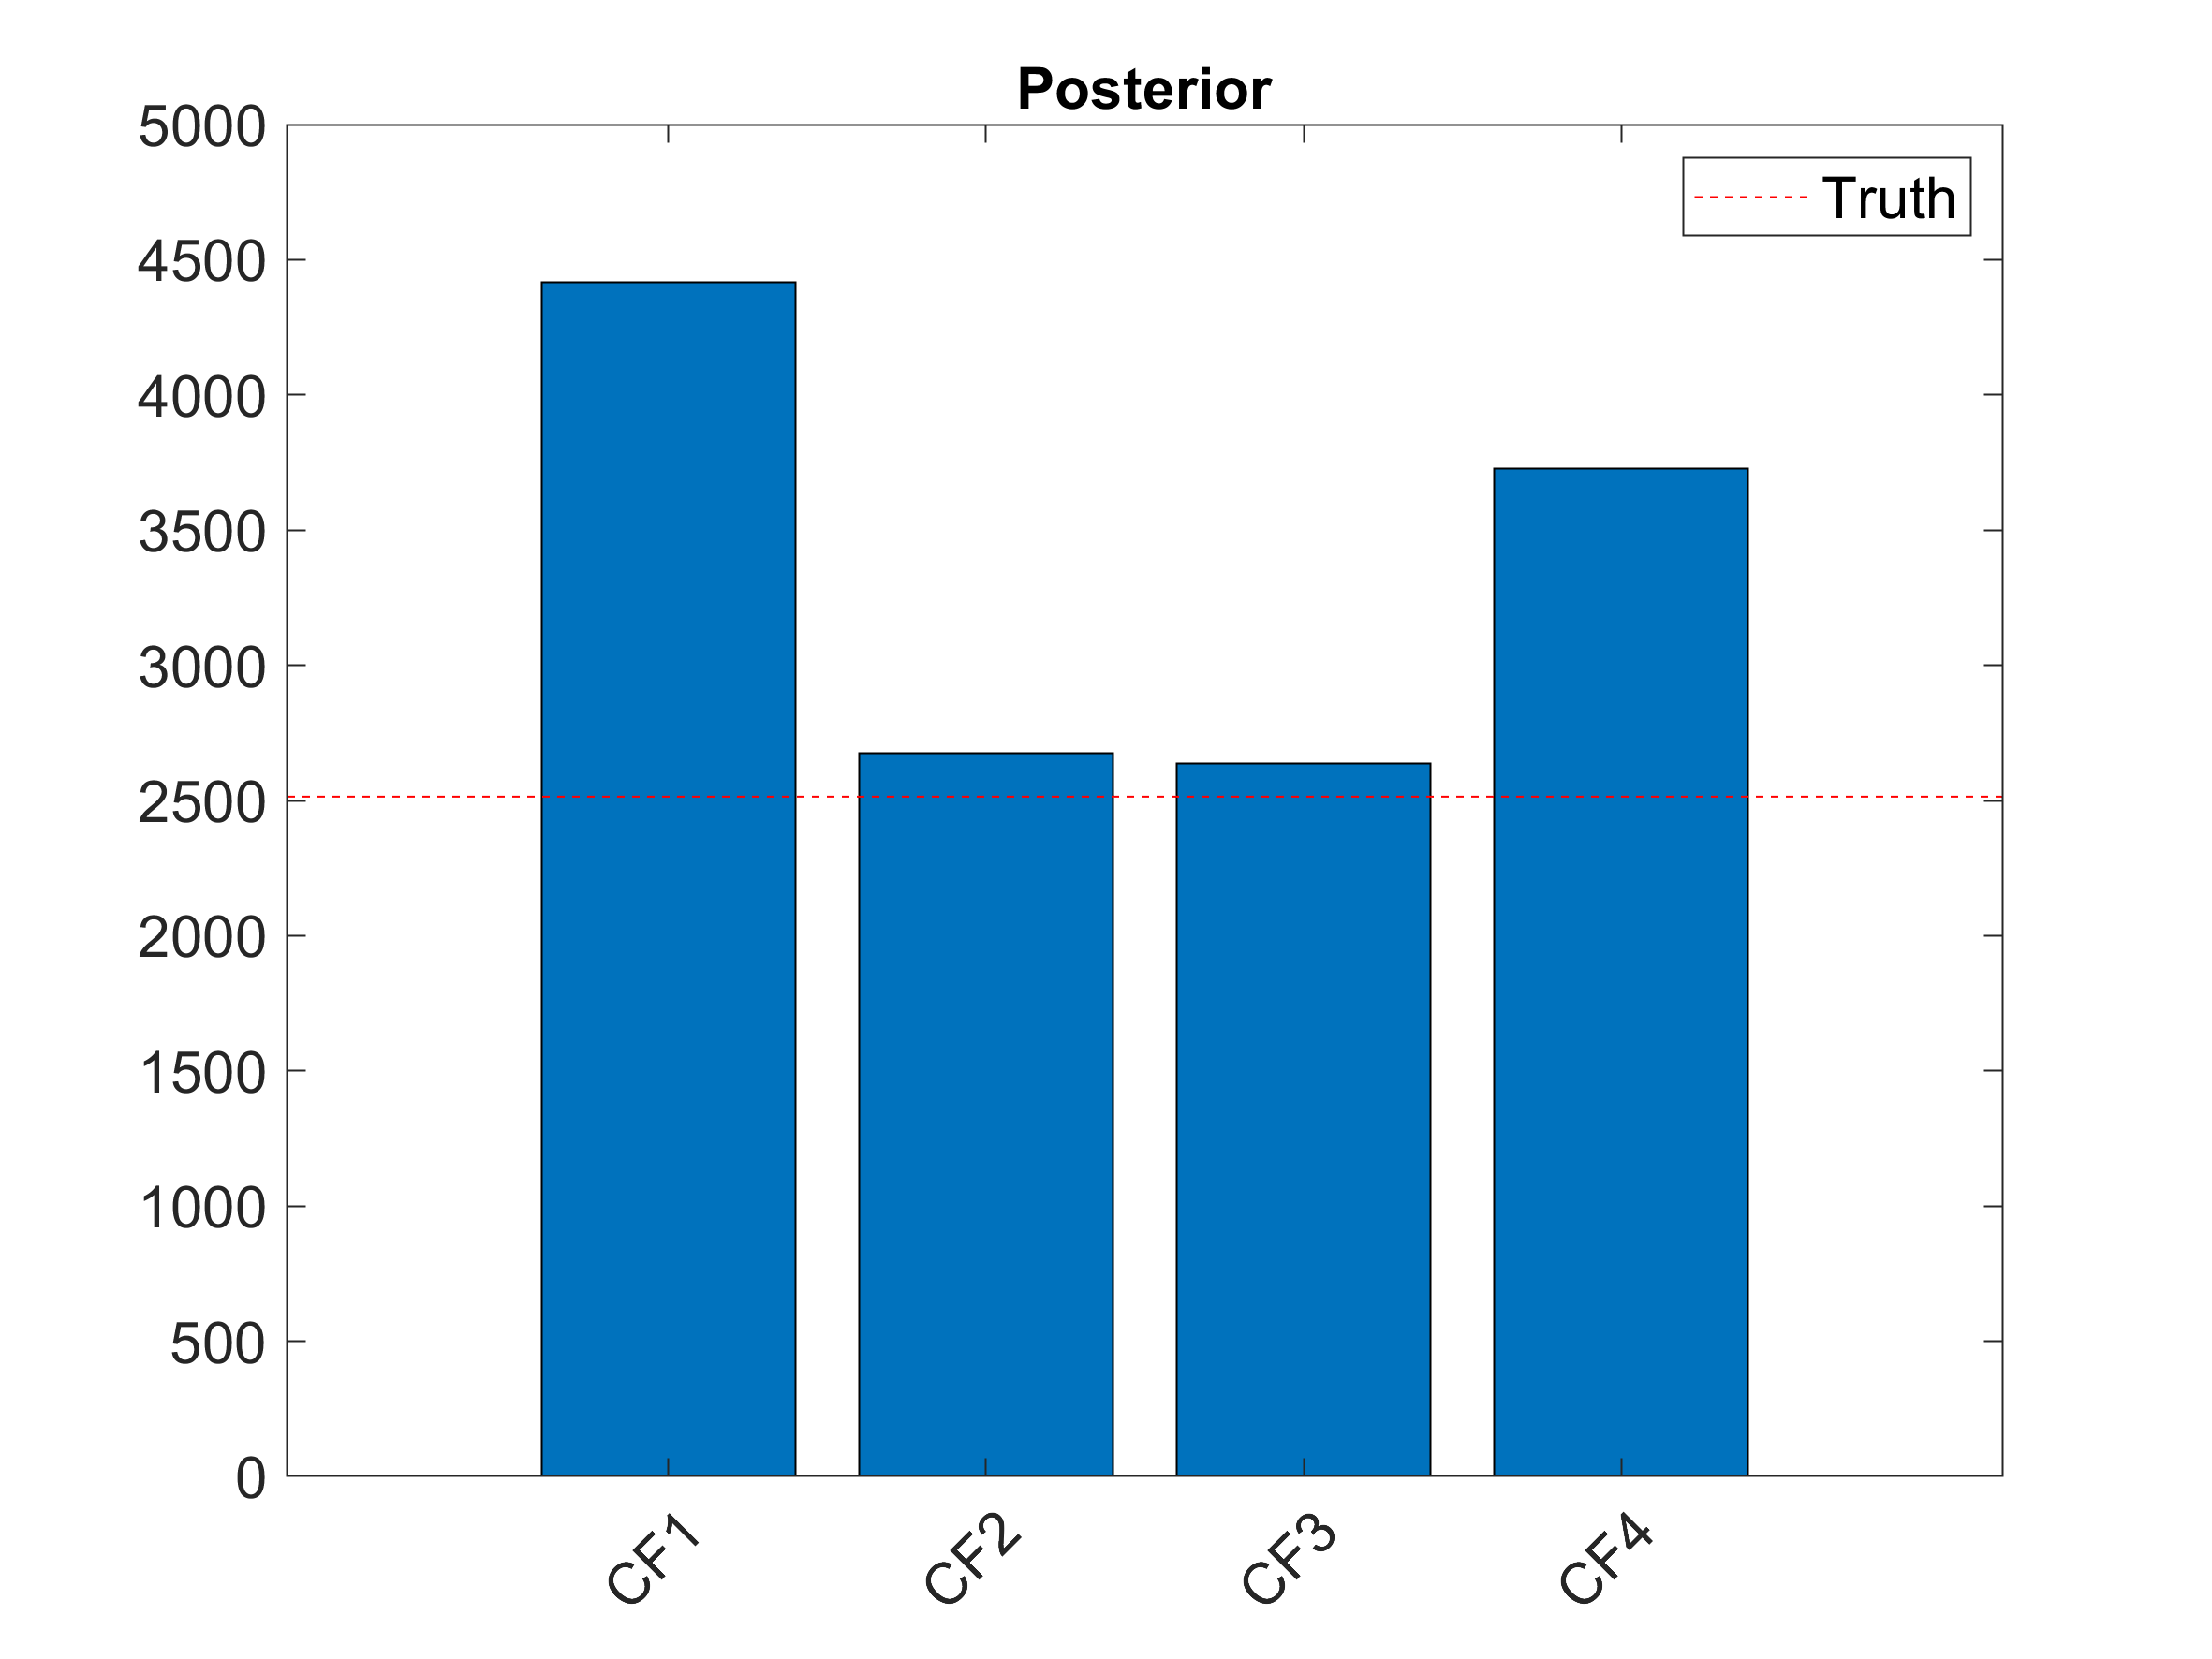
\includegraphics[width=0.8\textwidth]{./figures/res4.png}
	\caption{Blob detection result. Blobs are detected where the local maximas are detected.}
\end{figure}
\begin{figure}[htbp]
	\centering
	\includegraphics[width=0.8\textwidth]{./figures/res5.png}
	\caption{Blob detection result. Blobs are detected where the local maximas are detected.}
\end{figure}
\begin{figure}[htbp]
	\centering
	\includegraphics[width=0.8\textwidth]{./figures/res6.png}
	\caption{Blob detection result. Blobs are detected where the local maximas are detected.}
\end{figure}


	\begin{figure}[htbp]
		\centering
		\includegraphics[width=0.9\textwidth]{./figures/sift_matching.png}
		\caption{SIFT detection \& Matching Result.}
	\end{figure}
	\begin{figure}[htbp]
	\centering
	\includegraphics[width=0.9\textwidth]{./figures/projection.png}
	\caption{Compute $2$D similarity transformation using \textsc{RANSAC}. After $s,\mathbf{R,t}$ is obtained, transform SIFT features in image $1$ to image $2$.}
	\end{figure}
	\begin{figure}[htbp]
	\centering
	\includegraphics[width=0.9\textwidth]{./figures/blob_projection.png}
	\caption{Similar to previous image, but transform the blob detection results from image $1$ to image $2$. Red and blue circles denote the transformed and original detected blobs.}
\end{figure}
	\begin{figure}[htbp]
	\centering
	\includegraphics[width=0.9\textwidth]{./figures/hist.png}
	\caption{Histogram of the absolute difference of diameters. The majortiy of the absolute differences are within $5$ pixels.}
\end{figure}
%\begin{figure}
%	\centering
%	\includegraphics[width=0.9\textwidth]{./figures/a7.png}
%	\caption{Bacterial growth from movie frames. This is a snapshot of a single frame. See the complementary Gif for the animation.}
%	\includegraphics[width=0.7\textwidth]{./figures/a72}
%	\caption{Bacterial growth curve: assume one pixel equals to one bacteria.}
%\end{figure}
%\begin{figure}
%	\centering
%	\includegraphics[width=0.9\textwidth]{./figures/a7.png}
%	\caption{Bacterial growth from movie frames. This is a snapshot of a single frame. See the complementary Gif for the animation.}
%	\includegraphics[width=0.7\textwidth]{./figures/a72}
%	\caption{Bacterial growth curve: assume one pixel equals to one bacteria.}
%\end{figure}
%\begin{figure}
%	\centering
%	\includegraphics[width=0.9\textwidth]{./figures/a7.png}
%	\caption{Bacterial growth from movie frames. This is a snapshot of a single frame. See the complementary Gif for the animation.}
%	\includegraphics[width=0.7\textwidth]{./figures/a72}
%	\caption{Bacterial growth curve: assume one pixel equals to one bacteria.}
%\end{figure}
	\begin{table}
		\centering
		\caption{{Quantitative result of Assignment $3$}}
		\begin{tabular}{ccc}
			\hline
			\textbf{Image} &\textbf{Mean Diameters} & \textbf{Std of Diameters}  \\ \hline
			\textbf{CT\_lab\_high\_res} & $8.9411$ &   $6.8761$   \\ \hline
			\textbf{CT\_lab\_med\_res} & $7.6436$ &   $3.5724$  \\ \hline             
			\hline
		\end{tabular}
		\label{tb:mittest}
	\end{table}
	
	%\bibliography{PnPCites} 
	%\bibliographystyle{ieeetr}
	
\end{document}